Luego de correr todos los experimentos notamos que la direcci\'on IP de los nodos
no necesariamente refleja su posici\'on geogr\'afica real; esta es necesaria para
saber cuales ejes son intercontinentales, y por ende fijar un umbral $\bm{\mu}$ v\'alido.

~

Intentamos hacer uso de la herramienta www.geoiptool.com para orientarnos en
el curso de las rutas y algunas veces encontr\'abamos que no ten\'ian sentido las
ubicaciones que nos propon\'ia esta herramienta.

Un ejemplo de esto mismo seria:

~

\begin{tabular}{lll}
	\textit{\textbf{Host name}}	&	\textit{\textbf{IP}}	&	\textit{\textbf{RTT(media) ms}}	\\
	ET6-0-0-0-GRTBUECU1.red.telefonica-wholesale.net	&	94.142.103.153	&	30.104	\\
\end{tabular}

~

Dicha IP figura en geoiptool como localizada en Espa\~na. Es decir que de Buenos Aires, la ruta
pasar\'a por Espa\~na antes de llegar a Estados Unidos,
todo con un RTT medio de 30ms. Esto no parece para nada razonable, pero el nombre del host nos presenta informaci\'on que puede contrastar aquella
prove\'ida por geoiptool. GRT\textbf{BUE}CU1 indicar\'ia que la IP realmente pertenece a Buenos Aires, algo mucho m\'as l\'ogico.

Afortunadamente capturamos los nombres de los hosts en cada salto y la mayoria tiene indicios de ubicaci\'on en sus
nombres. Claro que no siempre encontramos hosts 'bien nombrados'.

~

Otro ejemplo podr\'ia ser \emph{be2384.ccr21.\textbf{lpl}01.atlas.cogentco.com} con el c\'odigo IATA de
Liverpool.

~

En las siguientes tablas se muestra la ubicaci\'on (no necesariamente aunque muy probablemente
correcta) del host en el que termina cada \textit{hop}, su IP, la media estad\'istica del Round Trip
Time a ese hop, y el Z-score de este host tomando como valor la diferencia de
tiempo con el host anterior. Como un paquete con TTL igual a 0 terminar\'ia en el cliente en un
tiempo inf\'initisamente chico, se toma el primer ``host'' con distancia 0.

Para simplificar las tablas y mejorar la comprensi\'on, en las tablas siguientes las filas correspondientes
a los links cuyos hosts est\'an en diferentes continentes (visto ``a ojo'') est\'an destacados.
Tambi\'en el link no-intercontinental con Z-score m\'as grande est\'a marcado, ya que va a ser
an\'alizado luego.

\subsection{Moscow State University (Rusia)}

\subsubsection{Ruta}

~

\begin{center}
\begin{tabular}{lllll}

	\textit{\textbf{Ubicaci\'on}}	&	\textit{\textbf{IP}}	&	\textit{\textbf{RTT(media) ms}}	&	\textit{\textbf{ZScore}}	\\
	Buenos Aires			&	200.51.240.181	&	31.018	&	0.220	\\
	Buenos Aires (telef\'onica)	&	94.142.103.153	&	30.104	&	-0.265	\\
	\intercontinental
	Miami (telef\'onica)		&	94.142.123.22	&	164.933	&	1.795	\\
	Dallas (telef\'onica)		&	94.142.127.105	&	199.813	&	0.278	\\
	Dallas/Ft Worth (cogentco)	&	154.54.13.225	&	221.383	&	0.077	\\
	Dallas/Ft Worth (cogentco)	&	154.54.7.45	&	212.266	&	-0.389	\\
	Kansas (cogentco)		&	154.54.2.113	&	214.954	&	-0.210	\\
	Chicago (cogentco)		&	154.54.6.86	&	215.663	&	-0.240	\\
	Toronto (cogentco)		&	154.54.27.182	&	228.466	&	-0.056	\\
	Montreal (cogentco)		&	154.54.30.206	&	226.107	&	-0.286	\\
	\intercontinental
	Liverpool (cogentco)		&	154.54.44.138	&	294.383	&	0.785	\\
	Amsterdam (cogentco)		&	154.54.77.245	&	307.648	&	-0.049	\\
	Hamburgo (cogentco)		&	154.54.74.122	&	264.320	&	-0.908	\\
	Estocolmo (cogentco)		&	154.54.63.2	&	327.827	&	\highestcontinental 0.713	\\
	Helsinki (cogentco)		&	154.54.62.250	&	332.424	&	-0.181	\\
	Mosc\'u				&	149.6.58.42	&	333.589	&	-0.233	\\
	Mosc\'u (runnet)		&	194.85.40.229	&	525.315	&	2.658	\\
	Mosc\'u (runnet)		&	194.190.254.118	&	357.420	&	-2.798	\\
	Mosc\'u (runnet)		&	93.180.0.172	&	344.003	&	-0.454	\\
	Mosc\'u				&	188.44.33.1	&	346.421	&	-0.214	\\
	Mosc\'u				&	188.44.50.103	&	347.007	&	-0.242	\\

\end{tabular}
\end{center}

~

Las ciudades fueron atravesadas en el siguiente orden:

Buenos Aires $\rightarrow$ Miami $\rightarrow$ Dallas $\rightarrow$ Kansas $\rightarrow$ Chicago
$\rightarrow$ Toronto $\rightarrow$ Montreal $\rightarrow$ Liverpool $\rightarrow$ Amsterdam
$\rightarrow$ Hamburg $\rightarrow$ Stockolm $\rightarrow$ Helsinki $\rightarrow$ Moscow

~

Como se puede ver, la conexi\'on primero pasa por varios hosts en los Estados Unidos y en Canad\'a antes de
pasar por un cable trans\'atlantico entre Montreal y Liverpool. A pesar de que estos dos son por lejos
los links m\'as largos, el link con Z-score m\'as alto es el que entra a la red en Mosc\'u. Esto se puede
deber a que los routers que administran internet dan mucha menos prioridad a paquetes ICMP que a paquetes que
solamente tienen que forwardear a su red. Por esta raz\'on, se puede ignorar sin consecuencias graves y tomar
al host siguiente con Z-score m\'as grande.

\begin{figure}[H]
	\begin{center}
		  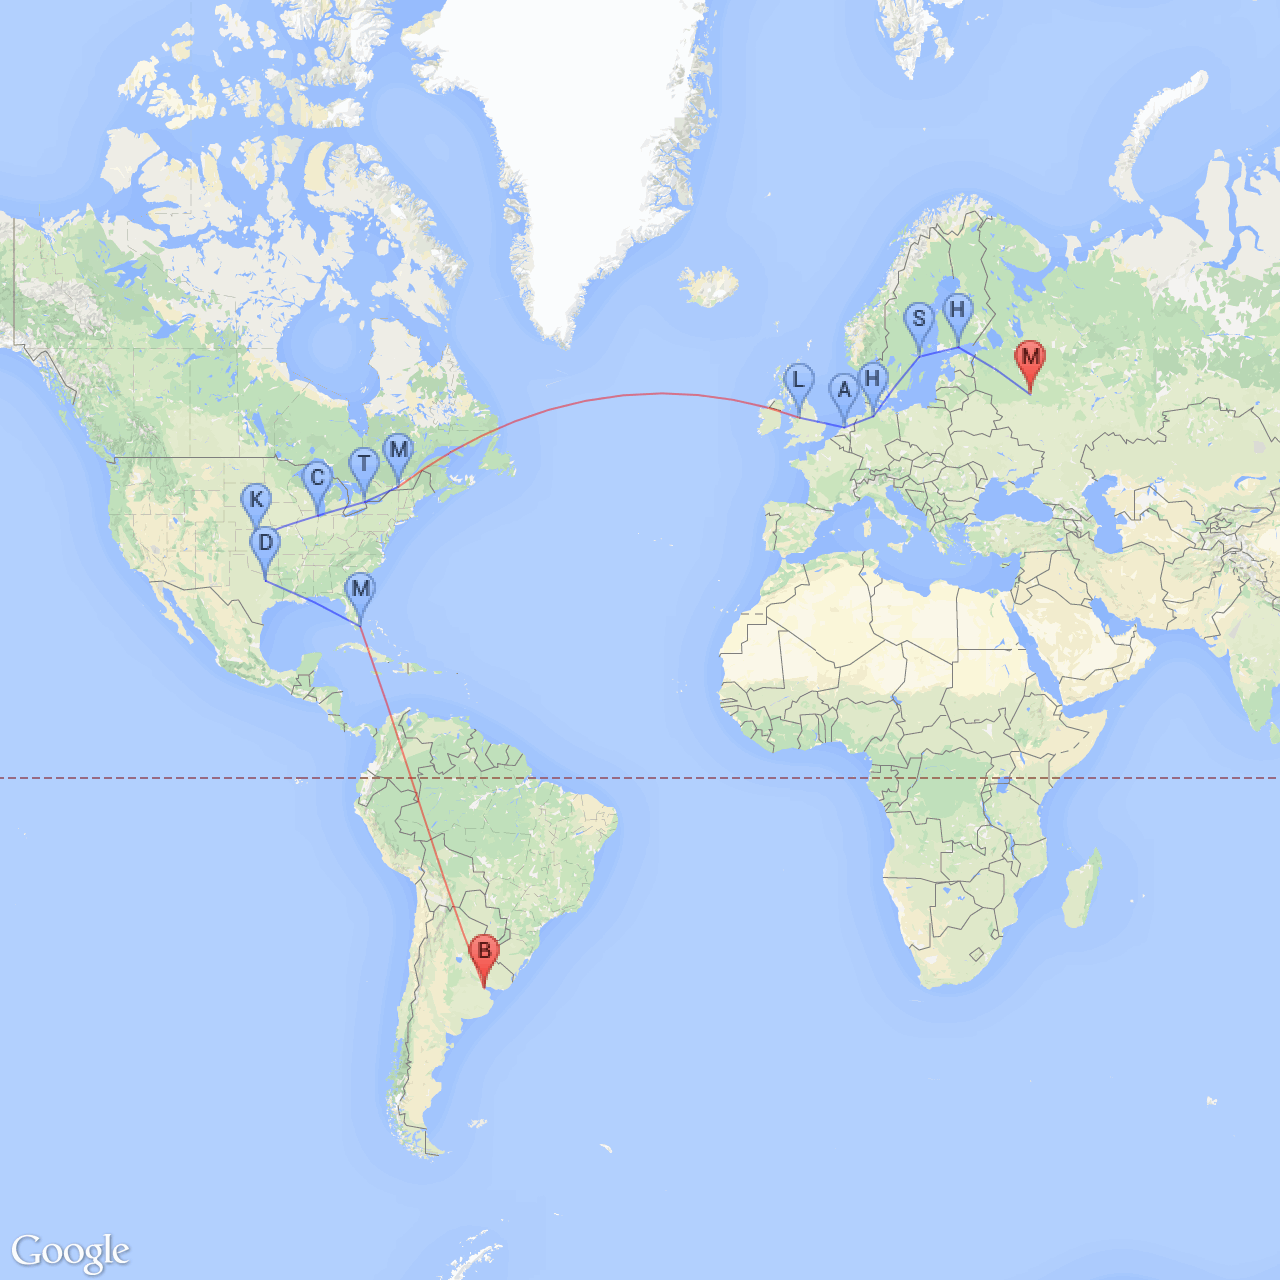
\includegraphics[scale=0.25]{../results/maps/MSU.png}
		  \caption{Mapa de la ruta atravesada para llegar a la universidad de Rusia}
	\end{center}
\end{figure}

\subsection{Tsinghua}

Para el caso de China, la ruta comienza por Estados Unidos como el caso anterior, pero en lugar de cruzar a Europa por el Este, los paquetes viajan por el pac\'ifico.
Veamos la siguiente tabla.

~

\begin{center}
\begin{tabular}{lllll}
	\textit{\textbf{Ubicaci\'on}}	&	\textit{\textbf{IP}}	&	\textit{\textbf{RTT(media) ms}}	&	\textit{\textbf{ZScore}}	\\
	Buenos Aires		&	(200.51.240.156)		&	31.907		&	0.276	\\
	Buenos Aires		&	(84.16.9.233)		&	30.095		&	-0.467	\\
	\intercontinental
	Miami		&	(94.142.121.222)		&	165.469		&	2.558	\\
	Miami		&	(94.142.122.249)		&	165.140		&	-0.434	\\
	Miami		&	(84.16.12.238)		&	167.934		&	-0.365	\\
	Miami		&	(63.243.152.45)		&	164.176		&	-0.510	\\
	Ashburn		&	(66.198.154.177)		&	215.945		&	\highestcontinental 0.714	\\
	Dallas		&	(66.198.154.118)		&	254.661		&	0.427	\\
	Dallas		&	(66.110.56.6)		&	267.287		&	-0.149	\\
	Los Angeles		&	(66.110.57.82)		&	256.103		&	-0.674	\\
	Los Angeles		&	(66.110.59.182)		&	257.170		&	-0.403	\\
	\intercontinental
	Chongming		&	(101.4.117.213)		&	428.694		&	3.355	\\
	Chongming		&	(101.4.117.97)		&	428.055		&	-0.441	\\
	Beijing		&	(101.4.116.146)		&	424.990		&	-0.495	\\
	Beijing		&	(101.4.118.78)		&	427.001		&	-0.383	\\
	Beijing		&	(202.112.38.10)		&	425.663		&	-0.456	\\
	Beijing		&	(118.229.4.66)		&	425.672		&	-0.427	\\
	Beijing		&	(118.229.4.34)		&	438.217		&	-0.150	\\
	Beijing		&	(118.229.2.74)		&	430.018		&	-0.608	\\
	Beijing		&	(118.229.2.69)		&	425.922		&	-0.517	\\
	Beijing		&	(118.229.8.6)		&	427.147		&	-0.400	\\
	Beijing (Tsinghua)		&	(166.111.4.100)		&	426.084		&	-0.450	\\
\end{tabular}
\end{center}

~

Las ciudades fueron atravesadas en el siguiente orden:

Buenos Aires $\rightarrow$ Miami $\rightarrow$ Ashburn $\rightarrow$ Dallas $\rightarrow$ Los
\'Angeles $\rightarrow$ Chongming $\rightarrow$ Beijing

~

El link continental m\'as largo, en Ashburn, tiene un Z-score de 0.714. Aunque es claramente un
outlier, lo podemos usar para la medici\'on de $\bm{\mu}$. El link intercontinental m\'as corto
tiene un Z-score de 2.558.

\begin{figure}[H]
	\begin{center}
		  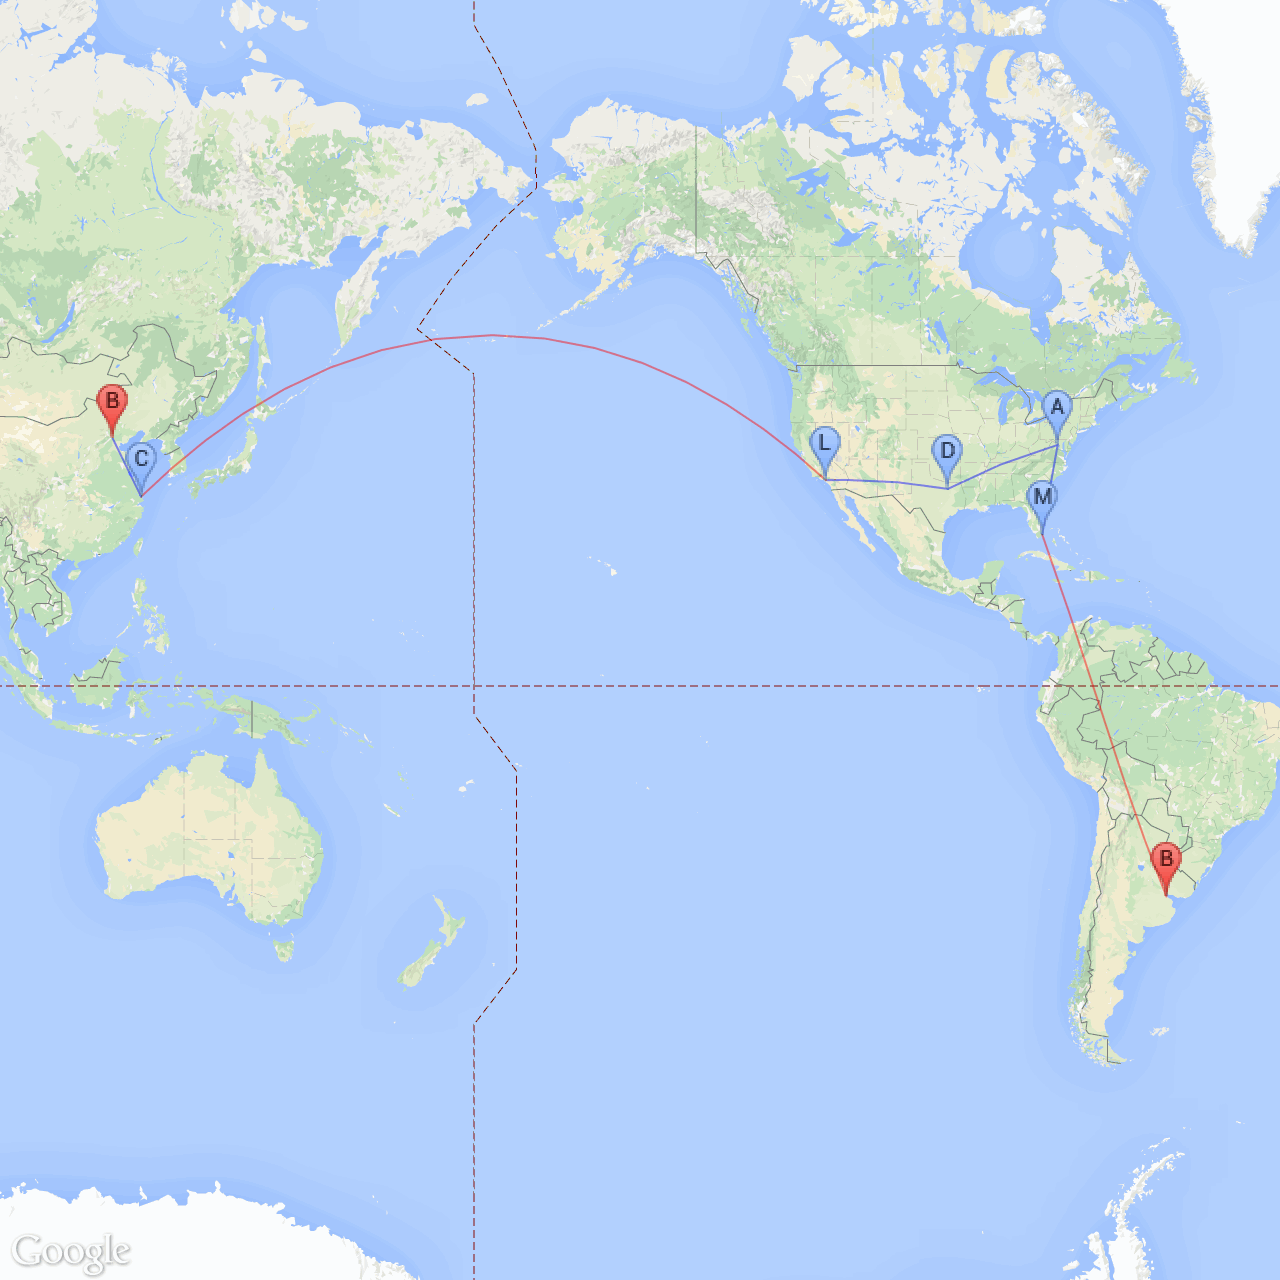
\includegraphics[scale=0.25]{../results/maps/Tsinghua.png}
		  \caption{Mapa de la ruta atravesada para llegar a la universidad de China}
	\end{center}
\end{figure}

\subsection{Oxford}

~

\begin{center}
\begin{tabular}{lllll}
	\textit{\textbf{Ubicaci\'on}}	&	\textit{\textbf{IP}}	&	\textit{\textbf{RTT(media) ms}}	&	\textit{\textbf{ZScore}}	\\
	Buenos Aires		&	(200.51.240.181)		&	37.154		&	0.454	\\
	Buenos Aires		&	(84.16.9.233)		&	51.008		&	-0.010	\\
	\intercontinental
	Miami		&	(5.53.5.138)		&	210.915		&	2.899	\\
	Miami		&	(94.142.123.5)		&	174.734		&	-1.006	\\
	Miami		&	(63.243.152.45)		&	175.240		&	-0.276	\\
	Ashburn		&	(66.198.154.177)		&	210.857		&	0.424	\\
	Ashburn		&	(216.6.87.1)		&	286.600		&	\highestcontinental 1.223	\\
	Newark		&	(216.6.87.138)		&	277.667		&	-0.464	\\
	Newark		&	(66.198.70.1)		&	307.315		&	0.305	\\
	\intercontinental
	Londres		&	(66.198.70.26)		&	403.133		&	1.622	\\
	Londres		&	(80.231.130.42)		&	298.757		&	-2.365	\\
	Londres		&	(195.219.100.82)		&	285.687		&	-0.546	\\
	Londres		&	(146.97.33.2)		&	289.063		&	-0.219	\\
	Londres		&	(146.97.37.206)		&	291.484		&	-0.238	\\
	Londres		&	(193.63.108.129)		&	281.783		&	-0.479	\\
	Londres		&	(193.63.108.134)		&	294.226		&	-0.038	\\
	Londres		&	(193.63.109.114)		&	289.814		&	-0.374	\\
	Londres		&	(192.76.21.21)		&	280.879		&	-0.464	\\
	Londres		&	(192.76.22.201)		&	282.251		&	-0.259	\\
	Londres		&	(192.76.32.66)		&	286.466		&	-0.202	\\
	Londres (Oxford)		&	(129.67.242.155)		&	301.388		&	0.011	\\
\end{tabular}
\end{center}

~

Las ciudades fueron atravesadas en el siguiente orden:

Buenos Aires $\rightarrow$ Miami $\rightarrow$ Ashburn $\rightarrow$ Newark $\rightarrow$ London $\rightarrow$ Oxford

~

En este caso el link a Ashburn tambi\'en es el que tiene el Z-score m\'as alto entre los links
continentales con 1.223, mientras que el link intercontinental m\'as bajo es de 1.622.

\begin{figure}[H]
	\begin{center}
		  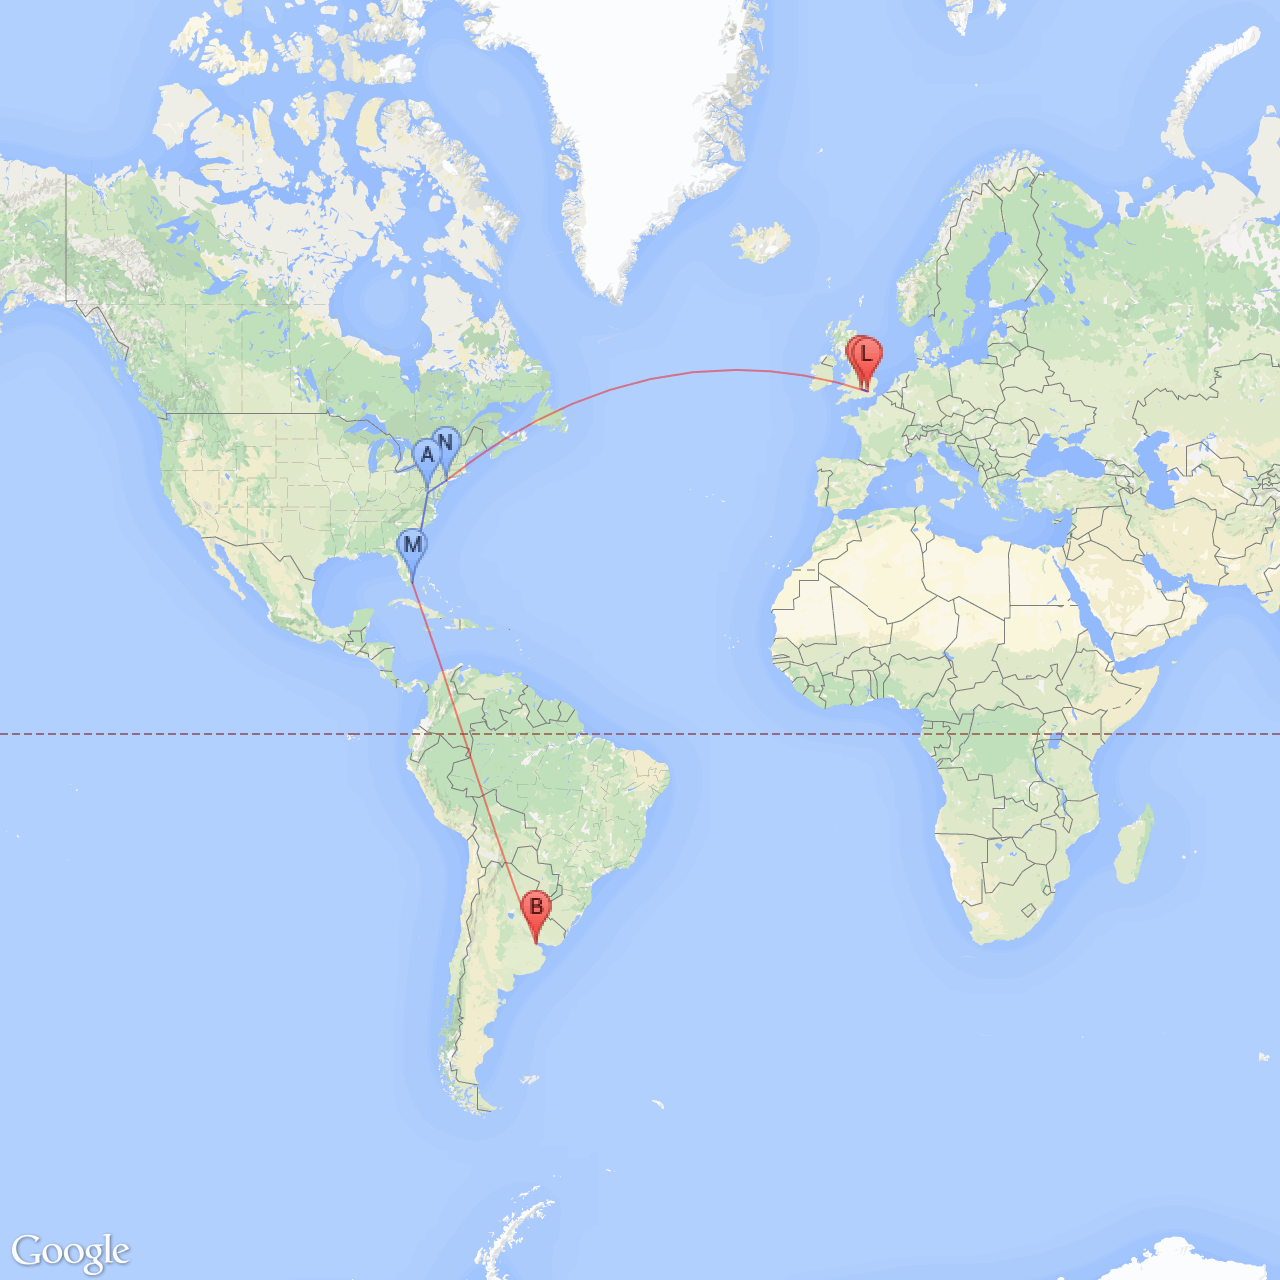
\includegraphics[scale=0.25]{../results/maps/Oxford.png}
		  \caption{Mapa de la ruta atravesada para llegar a la universidad de Inglaterra}
	\end{center}
\end{figure}

\subsection{Queensland}

~

\begin{center}
\begin{tabular}{llllll}
	\textit{\textbf{Ubicaci\'on}}	&	\textit{\textbf{IP}}	&	\textit{\textbf{RTT(media) ms}}	&	\textit{\textbf{ZScore}}	\\
		Buenos Aires		&	(200.51.240.156)		&	31.896		&	0.140	\\
		Buenos Aires		&	(84.16.9.233)		&	30.748		&	-0.509	\\
		\intercontinental
		Miami		&	(94.142.123.14)		&	165.811		&	2.170	\\
		??? (213.140.49.13)		&	(213.140.49.13)		&	230.069		&	\highestcontinental 0.776	\\
		Palo Alto		&	(64.125.13.113)		&	229.511		&	-0.497	\\
		\intercontinental
		Sydney		&	(208.185.52.74)		&	392.486		&	2.720	\\
		Sydney		&	(202.158.194.176)		&	391.129		&	-0.513	\\
		Sydney		&	(113.197.15.57)		&	419.913		&	0.079	\\
		Brisbane		&	(202.158.194.54)		&	407.555		&	-0.729	\\
		Brisbane		&	(202.158.194.213)		&	394.376		&	-0.745	\\
		Queensland		&	(202.158.209.3)		&	394.951		&	-0.475	\\
		Queensland		&	(113.197.8.34)		&	391.479		&	-0.555	\\
		Queensland		&	(130.102.159.1)		&	392.041		&	-0.475	\\
		Queensland		&	(130.102.0.242)		&	401.994		&	-0.291	\\
		Queensland		&	(130.102.82.28)		&	403.280		&	-0.461	\\
		Queensland		&	(130.102.131.70)		&	396.128		&	-0.627	\\
\end{tabular}
\end{center}

~

Las ciudades fueron atravesadas en el siguiente orden:
Buenos Aires $\rightarrow$ Miami $\rightarrow$ Hermosa Beach $\rightarrow$ Sydney $\rightarrow$ Brisbane $\rightarrow$ Queensland

Aqu\'i el link continental con mayor Z-score tiene uno de 2.720, mientras que el link continental con mayor
Z-score es de 0.776.

~

\begin{figure}[H]
	\begin{center}
		  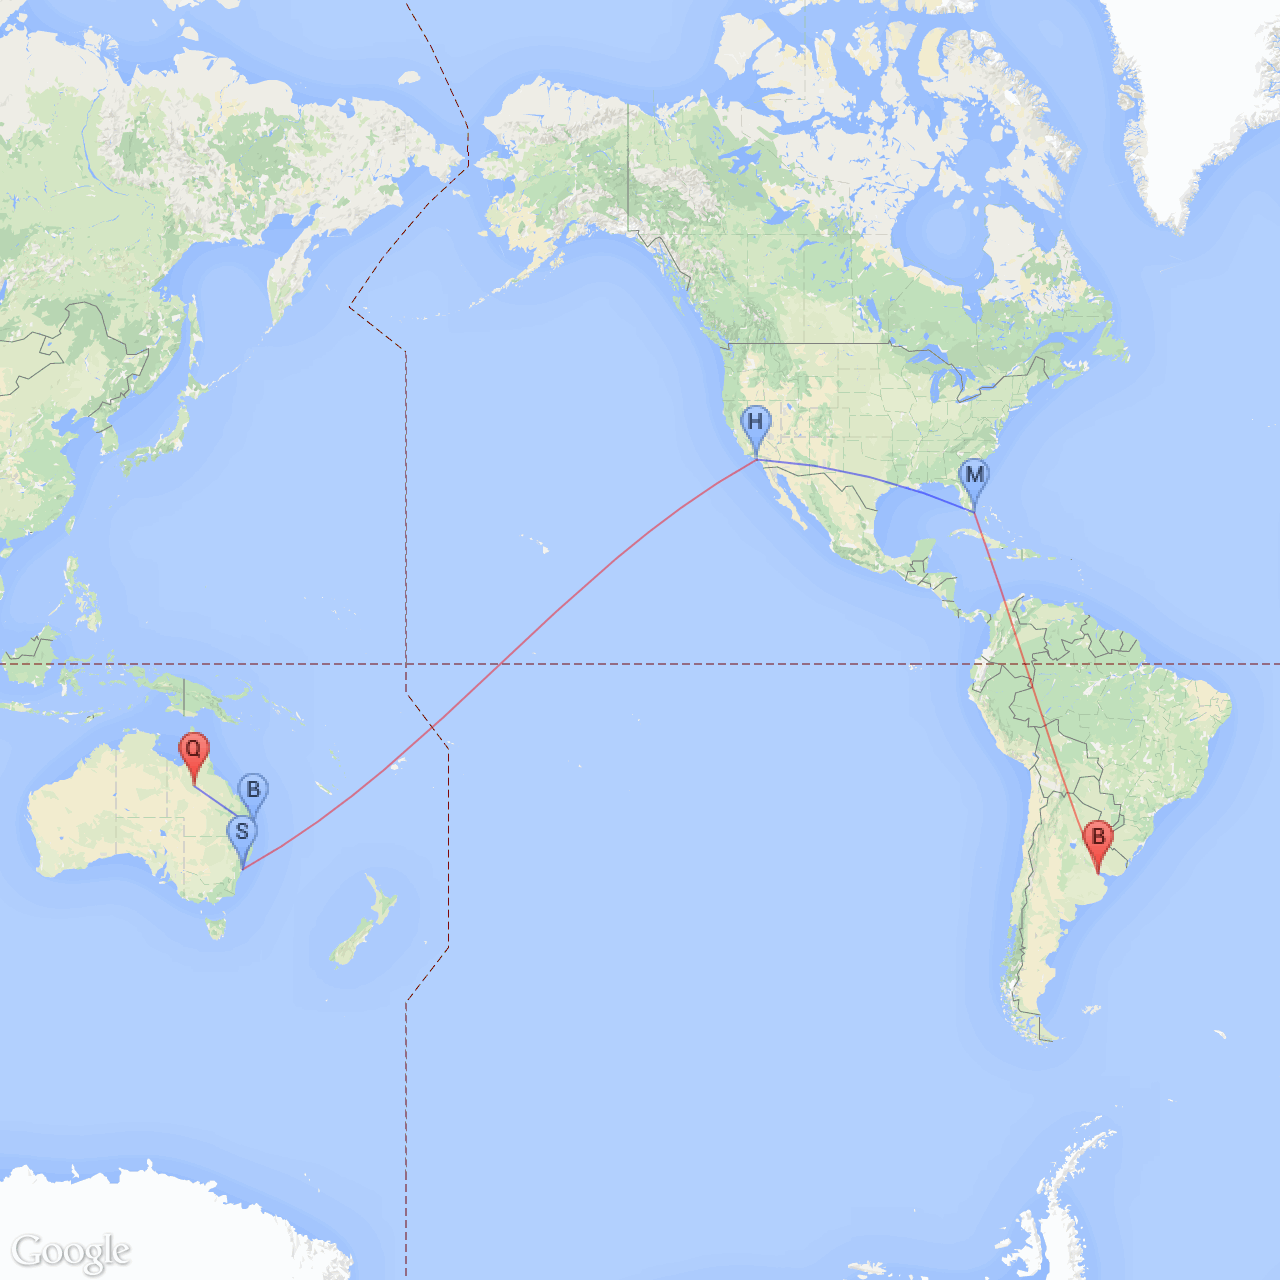
\includegraphics[scale=0.25]{../results/maps/Queensland.png}
		  \caption{Mapa de la ruta atravesada para llegar a la universidad de Australia}
	\end{center}
\end{figure}

Entre todos los hosts, el link intercontinental con Z-score m\'as bajo es el de Montreal a
Liverpool, con $Z_{rtt} = 0.785$, mientras que el link intracontinenteal con Z-score m\'as alto es
uno de un host a otro en la ciudad as Ashburn, con $Z_{rtt} = 1.233.
